\documentclass[]{report}   
\usepackage{amsmath} 
\usepackage{pdfpages}
\usepackage{lipsum}
\usepackage{graphicx}
\usepackage{float}

\newcommand{\tab}{\hspace*{2em}}

\begin{document}

\title{Title}   
\author{\makebox[\linewidth][c]{Author 1\tab Author 2\tab Author 3}}         

\maketitle

\begin{abstract}
	\lipsum[1] 
\end{abstract}

\tableofcontents

% chapter 1
\chapter{UML Data Model}    
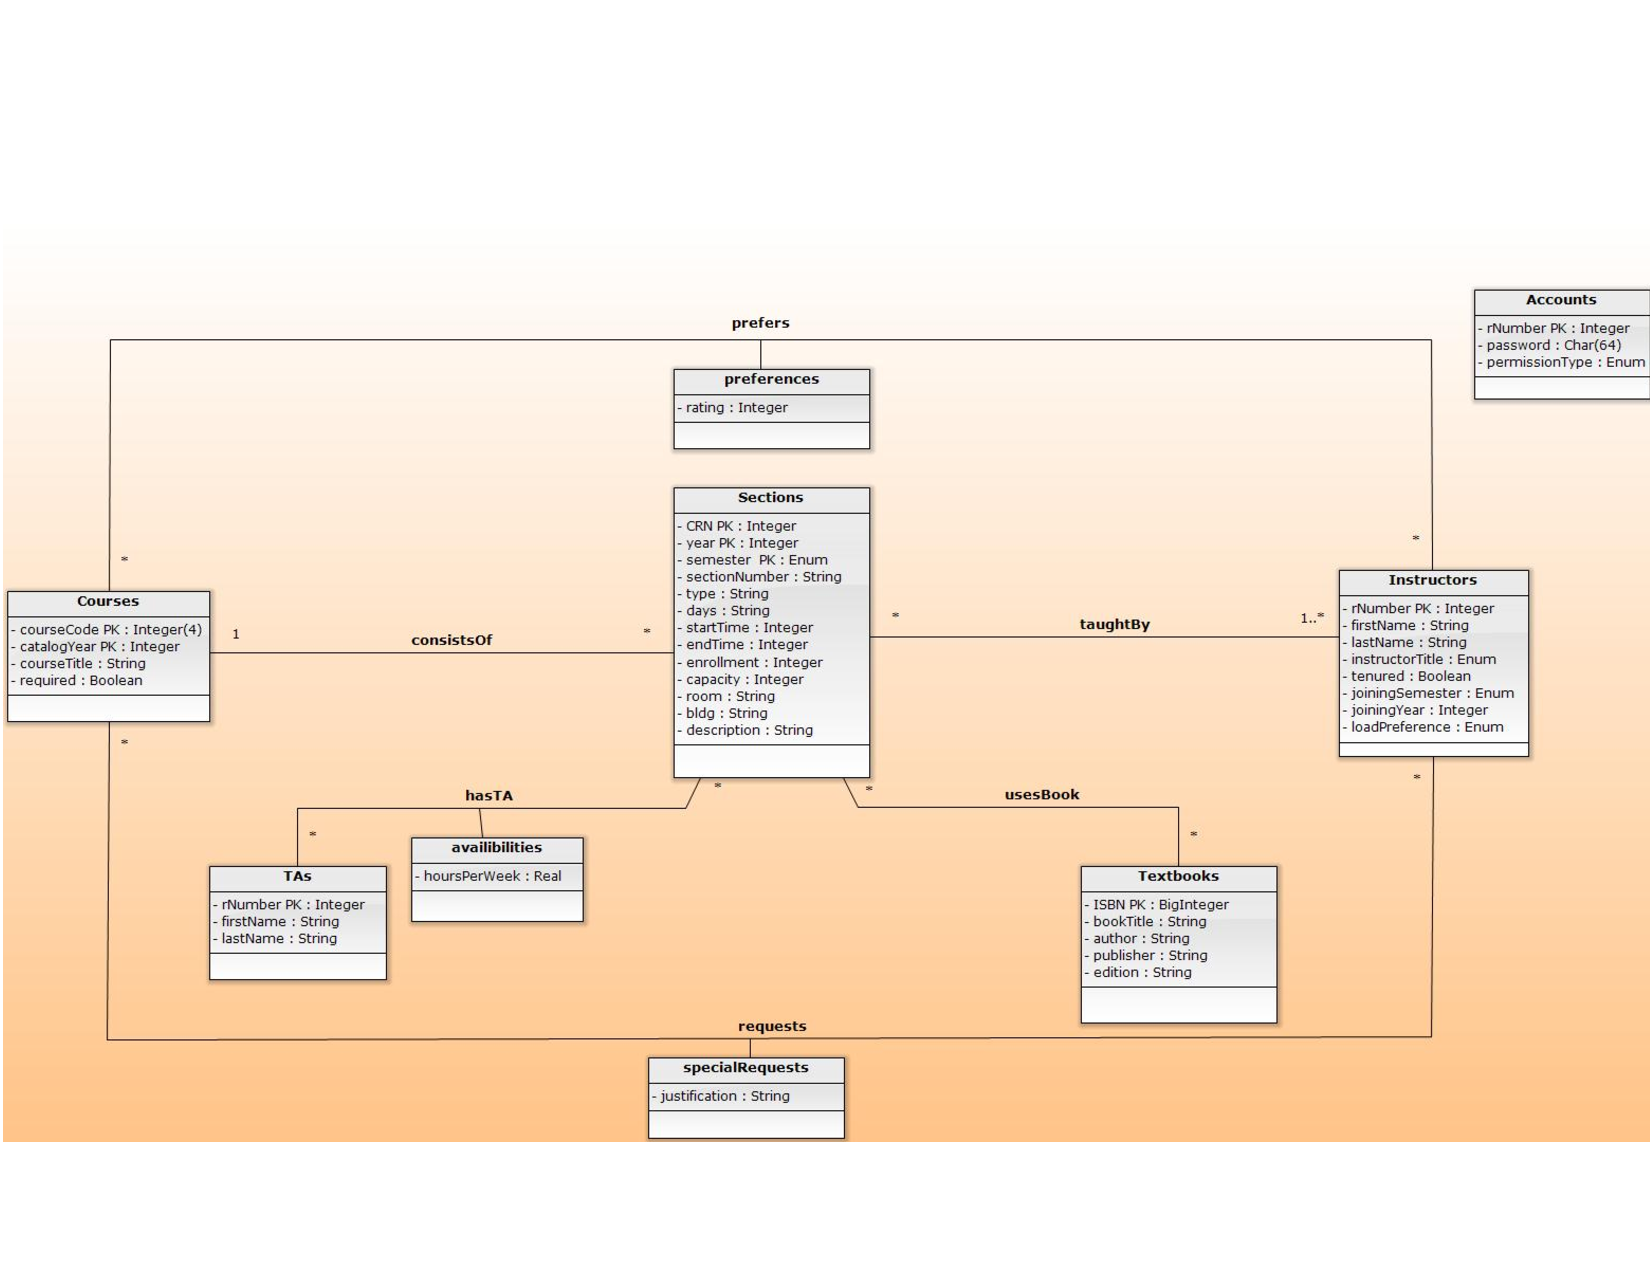
\includepdf[landscape]{umldiagram.pdf}

\chapter{Relation Schemas}
%Courses Table
\section{Courses}
	Courses(\underline{courseCode}, \underline{catalogYear}, courseTitle, required) 
		Tuples in the Courses table contain information about a given course during a specific catalog year.

	\subsection{courseCode}
		PK : int 
		Four digit numerical identifier for a class that is given at Texas Tech University. This code is used to represent all classes of this type. There may be many sections that share a course code in a given semester. (e.g. 4000)	
		
	\subsection{catalogYear}
		PK : int(4) 
		Four digit numerical identifier for a catalog year. The first two digits represent the year that the catalog begins in and the final two digits represent the year that the catalog ends in. (e.g. We represent the academic year of 2014-2015 as 1415)
		
	\subsection{courseTitle}	
		: str 
		The description of the class referred to by this tuple.
		
	\subsection{required}
		: boolean
		Whether or not this class is required for a degree in Computer Science (e.g. true = required, false = not required).
	
	
%Sections Table
\section{Sections}
	Sections(\underline{CRN}, \underline{year}, \underline{semester}, sectionNumber, type, days, startTime, endTime, enrollment, capacity, room, bldg) 
		Tuples in the Section table contain information for a unique section of a course.

	\subsection{CRN}
		PK : int  
		Unique ID for the section in a given year.
	
	\subsection{year}
		PK : int (1920 $<$ x $<$ 3000) 
		Year the section is being offer.
		
	\subsection{semester}
		PK : enum (Fall/Spring/Summer I/Summer II)
		Semester the section is being offer.
	
	\subsection{sectionNumber}
	 	: str 
		The unique number of the section.
	
	\subsection{type}
	 	:str 
		Teaching method of the section (e.g. online, in-class and lab).   
	
	
	\subsection{days}
		: str 
		Days the section meets. (e.g. MWF means the class will meet Monday, Wednesday and Friday)
	
	\subsection{startTime}
		: int (0000 $\leq$ x $<$ 2400)
		Time the section starts, the use of military time is for data storage efficiency and accuracy. Twelve hour time will be display for the user.
	
	\subsection{endTime}
	 	: int (0000 $\leq$ x $<$ 2400) 
		Time the section ends, the use of military time is for data storage efficiency and accuracy. 12 hour time will be display for the user.
	
	\subsection{enrollment}
		: int  
		Number of students enroll in the section.
	
	\subsection{capacity}
		: int
		Maximum number of students can enroll in the section according to the department. 
	\subsection{room}
		: str
		The room number where the class is going to be located.
		    	
	\subsection{bldg}
		: str
		The building where the class is going to be located.
		
	\subsection{descriptions}
		: str
		The title of a special topics or special project course.
		    


%Instructors Table
\section{Instructors}
	Instructors(\underline{rNumber}, lastName, firstName, instructorTitle, tenured, joiningSemester, joiningYear, loadPreference) 
		Tuples in the Instructors table contain information for instructors.
	
	\subsection{rNumber}
		PK: int
		Unique numerical identifier for students, staff, and professors at Texas Tech University.
    
    \subsection{lastName}
		: str  
    	The last name of the instructor.
    
    \subsection{firstName}
    	: str 
    	The first name of the instructor.
  
    \subsection{instructorTitle}
    	: str (Professor/FTI/GPTI/Null)
    	Title of the instructor.
    
    \subsection{tenured}    
    	: boolean 
    	Represents if the instructor is tenured or not.
    
    \subsection{joiningSemester}
    	: str (Fall/Spring/Summer I/Summer II) 
    	The semester in which the instructor joined the college.
    
    \subsection{joiningYear}
    	: int (1920 $<$ x $<$ 3000 )
    	The year in which the instructor joined the college. Must be greater than 0 and less than 3000.
    
    \subsection{loadPreference}
    	: str (Spring/Fall/NULL)
    	The semester in which the instructor prefers to teach more. NULL for no preference.
    	
    
%TAs Table
\section{TAs}
	TAs(\underline{rNumber}, lastName, firstName)
		Tuples in the TAs table represent information about a particular teaching assistant.

	\subsection{rNumber}
		PK : int 
		Unique numerical identifier for students, staff, and professors at Texas Tech University.
		
	\subsection{lastName}
		: str  
    	The last name of the teacher assistant.
    
    \subsection{firstName}
    	: str 
    	The first name of the teacher assistant.
	
%Textbooks Table
\section{Textbooks}
	Textbooks(\underline{ISBN}, bookTitle, author, publisher, edition) 
		Tuples in the Textbooks table contain information for books used in a Course

	\subsection{ISBN}
		PK : big int
		Unique numerical identifier for textbooks.
	
	\subsection{bookTitle}
		: str 
		Title of the textbook
	
	\subsection{author}
		: str 
		Name of the textbook author
	
	\subsection{publisher}
		: str 
		Publisher of the textbook
	
	\subsection{edition}
		: str 
		Edition of the Textbook


%consistsOf Table
\section{consistsOf}
	consistsOf(\underline{CRN}, \underline{semester}, \underline{year}, courseCode, catalogYear) 
		Tuples in the consistOf table contain information for relation between a course and a section.
	
	\subsection{CRN}
		PK: int 
		Unique ID for the section in a given year.

	\subsection{semester}
		PK : enum (Fall/Spring/Summer I/Summer II)
		Semester the section is being offer.
	
	\subsection{year}
		PK : int (1920 $<$ x $<$ 3000)
		Year the section is being offer.
	
	\subsection{courseCode}
		: int
		Four digit numerical identifier for a class that is given at Texas Tech University. This code is used to represent all classes of this type. There may be many sections that share a course code in a given semester. (e.g. 4000)
	
	\subsection{catalogYear}
		PK : int(4) 
		Four digit numerical identifier for a catalog year. The first two digits represent the year that the catalog begins in and the final two digits represent the year that the catalog ends in. (e.g. We represent the academic year of 2014-2015 as 1415)


%taughtBy Table
\section{taughtBy}
	taughtBy(\underline{CRN}, \underline{semester}, \underline{year}, \underline{rNumber}) 
		Tuples in the taughtBy table contain information for relation between instructor and section of a course.
 	
 	\subsection{CRN}
		PK: int 
		Unique ID for the section in a given year.
		
	\subsection{semester}
		PK : enum (Fall/Spring/Summer I/Summer II)
		Semester the section is being offer.
	
	\subsection{year}
		PK : int (1920 $<$ x $<$ 3000) 
		year the section is being offer.
	
	\subsection{rNumber}
		PK : int 
		Unique numerical identifier for students, staff, and professors at Texas Tech University.


%HasTA Table
\section{HasTA}
	HasTA(\underline{CRN}, \underline{semester}, \underline{year}, \underline{rNumber}, hoursPerWeek) 
		Tuples in the HasTA table represent a TA being associated with (assisting) a particular section of a course.
	
	\subsection{CRN}
		PK : int 
		The CRN of the course the TA is assisting (cf. Section).
	
	\subsection{semester}
		PK : enum (Fall/Spring/Summer I/Summer II)
		Semester the section is being offer.
			
	\subsection{year}
		PK : int 
		The year of the course the TA is assisting (cf. Section). Since CRN and year are the keys for the Section table, they are sufficient to determine which section of the course is being referred to.
	
	\subsection{rNumber}
		PK : int 
		Unique numerical identifier for students, staff, and professors at Texas Tech University.
	
	\subsection{hoursPerWeek}
		: real 
		The number of hours each week the TA is available to help (e.g. 16.5).


%usesBook Table
\section{usesBook}
	usesBook(\underline{CRN}, \underline{semester}, \underline{year}, \underline{ISBN}) 
		The usesBook relation gives a description of the textbook that is associated with a given class.
	
	\subsection{CRN}
 		PK : int 
 		is classified as an int due to it being a collection of only numbers associated with one particular class. The CRN will reference the CRN in the relation sections, and it is in this relation due to this one particular class associated with this unique number will then uniquely use a particular textbook.
	
	\subsection{semester}
		PK : enum (Fall/Spring/Summer I/Summer II)
		Semester the section is being offer.
		
	\subsection{year}
		PK : int 
		is classified as an int due to it being a collection of only numbers associated with a given school year. The year will reference the year in the relation sections, and its a unique key that depends on the CRN. The year is part of this relation due to it being in link with CRN since a CRN is dependent on the school year that a particular number can 	repeat.
	
	\subsection{ISBN}
 		PK : big int  
 		Unique numerical identifier for textbooks.
	
	
%prefers Table	
\section{prefers}
	prefers(\underline{rNumber}, \underline{courseCode}, \underline{catalogYear}, rating) 
		Tuples in the prefers table contain information for relation between a professor and a course preference.
	
	\subsection{rNumber}
		PK : int 
		Unique numerical identifier for students, staff, and professors at Texas Tech University.
	
	\subsection{courseCode}
		PK : int
		Four digit numerical identifier for a class that is given at Texas Tech University. This code is used to represent all classes of this type. There may be many sections that share a course code in a given semester. (e.g. 4000)
	
	\subsection{catalogYear}
		PK : int(4) 
		Four digit numerical identifier for a catalog year. The first two digits represent the year that the catalog begins in and the final two digits represent the year that the catalog ends in. (e.g. We represent the academic year of 2014-2015 as 1415)
	
	\subsection{rating}
		: int 
		Numerical ranking of 1, 2, 3, or null. Ranking represents an instructors desire to teach a course. 1 is the most desirable, followed by 2, then 3. A null value represents that an instructor does not wish to teach the course. 


%requests Table
\section{requests}
	requests(\underline{rNumber}, \underline{courseCode}, \underline{catalogYear}, justification) 
		Tuples in the requests table contain information for relation between a professor and any special request they might have for a course.
	
	\subsection{rNumber}
		PK : int
		Unique numerical identifier for students, staff, and professors at Texas Tech University.
	
	\subsection{courseCode}
		PK : int
		Four digit numerical identifier for a class that is given at Texas Tech University. This code is used to represent all classes of this type. There may be many sections that share a course code in a given semester. (e.g. 4000)
	
	\subsection{catalogYear}
		PK : int(4) 
		Four digit numerical identifier for a catalog year. The first two digits represent the year that the catalog begins in and the final two digits represent the year that the catalog ends in. (e.g. We represent the academic year of 2014-2015 as 1415)
	
	\subsection{justification}
		: str
		A variable length comment. Justification is a comment written by an instructor to state their justification for wanting (or not) to teach a specific course. 


%Accounts Table
\section{Accounts}
	Logins(\underline{rNumber}, password, permissionType) 
		Holds account information to control viewing and editing databases on the website.
	
	\subsection{rNumber}
		PK : int 
		Unique numerical identifier for students, staff, and professors at Texas Tech University.
    
    \subsection{password}
    	: char(64)
    	Used to validate the account.
    
    \subsection{permissionType}
	    : str(Faculty/Instructor/Business) 
		Determines what the user can view and edit.		
                   
\chapter{SQL Pseudocode}           
`\$' denotes user-input or gathered values from system. 

\section{Faculty}
\begin{enumerate}
	%1
	\item 	 A department faculty/staff can login and update the following information.
	\begin{enumerate}
		%1a
		\item	 When there is a new professor / FTI / GPTI joining the department, add the information of the new people into the system. The information including the joining date (which semester of which year, e.g., spring 2013), tenured or untenured, and title (e.g., assistant/associate/full professor). However for FTI/GPTI, we don’t have title or tenure information.\\
		
				\texttt{SELECT rNumber, lastName, firstName, title, tenured, joiningSemester, joiningYear\\ 
						FROM Instructors;}\\
						
				\texttt{INSERT INTO Instructors ( rNumber, firstName, lastName, instructorTitle, tenured, joiningSemester, joiningYear, loadPreference) VALUES ( \$rNumber, \$firstName, \$lastName, \$instructorTitle, \$tenured, \$joiningSemester, \$joiningYear, \$loadPreference );}\\
					
				Where \texttt{tenured} and \texttt{title} may be null for FTI/GPTI.
				This query inserts information about new instructors into the Instructor table. An instructor may include/update their load preference later.  
				

		%1b
		\item 	 For each semester and every section of an offered course, input who is the instructor, where and when the section is taught, the capacity limit of the section and the enrollment of this class. For example, for CS4354 section 001, time (10am to 10:50am) days (MWF), room (204), building (ENGCTR), capacity (60), and enrollment (35). Note that for a section of a course, there may be more than one
instructor.\\

				\texttt{INSERT INTO Sections\\
						VALUES (\$CRN, \$year, \$sectionNumber, \$type, \$semester, \$days, \$startTime, \$endTime, \$enrollment, \$capacity))}\\

				For each section of a course, a department faculty/staff can input the information for the section including CRN, year, section number, type of section, semester, days of the week the section meets, start time and end time of the section, enrollment, and capacity for the class. 

		%1c
		\item 	For each section of a course, input the TA/Grader name, and hours the TA/Grader will assist this course.\\

				Query to determine the courses to put in the dropdown:\\
				\texttt{SELECT distinct courseCode\\
						FROM consistsOf NATURAL JOIN Courses\\
						WHERE semester = \$semester AND year = \$year\\
						ORDER BY courseCode;}\\

				Query to fill the table with course information:\\
				\texttt{SELECT * \\
						FROM Sections NATURAL LEFT OUTER JOIN hasTA NATURAL LEFT OURTER JOIN TAs\\
						WHERE Sections.CRN IN (\\
							\tab SELECT CRN\\
							\tab FROM consistsOf\\
							\tab WHERE courseCode = \$course AND year=\$year AND semester=\%semester)\\
						AND Sections.year=\$year AND Sections.semester=\$semester;}\\

				
		%1d
		\item 	The course list of computer science. For each course, there is an attribute of catalog whose value is year. E.g., a course with catalog 2014 means that the course is a course in 2014 catalog.\\

				\texttt{SELECT courseCode , courseTitle \\
						FROM Courses\\
						WHERE catalogYear = '" . \$year . ( \$year + 1 ) . "';}\\
				
						Return a list of all course codes for a given catalog year, that is requested/entered by the user.  
			
	\end{enumerate}

\section{Instructor}
	%2
	\item 	A professor can login and do the following tasks
	\begin{enumerate}
		
		%2a
		\item 	Update her/his preferences of the courses to teach in a given academic year (e.g., Fall 2013 to Summer II 2014). As for the user interface, all courses will be displayed with the professor’s preference value (1-3) for that year (if the preference value is not there yet, use the previous year’s preference values). The professor can edit the values. A preference value of NULL represents that the corresponding course is not preferred by the professor.\\

				\texttt{INSERT INTO preferences\\
						VALUES (\$rNumber, \$courseCode, \$catalogYear, \$rating)}\\
						
						Store preferences for each instructor for each course and the year. 
		
		%2b
		\item 	Update her/his teaching load distribution (only in fall and spring) preference: more load in fall or more load in spring or don’t care\\

				\texttt{UPDATE Instructors\\
						SET loadPreference = \$loadPreference\\
						WHERE rNumber = \$rNumber}\\
						
						The instructor can update their load preference during the school year.
		
		%2c
		\item 	 Input special request for a given year: course code, title, justification ($<$200 words).\\
		
				\texttt{INSERT INTO Requests\\
						VALUES (\$rNumber, \$courseCode, \$catalogYear, \$justification)}\\	
						
		%2d 	
		\item	For each section of a course assigned to this professor in a given semester, input the text books with the following information: Text Title, Author, Edition, ISBN \#, Publisher. Here we assume the assignment of the given semester is already inside the database. If the course was taught before by this professor, the most recent text information should be displayed as the default text information.\\

				Query to determine the courses an instructor has for the semester:\\
				\texttt{SELECT distinct courseCode\\
						FROM consistsOf NATURAL JOIN Courses\\
						WHERE semester=\$semester AND year=\$year\\
						ORDER BY courseCode;}\\

				Query to fill the table with textbook information:\\
				\texttt{SELECT *\\
						FROM usesBook NATURAL JOIN taughtBy NATURAL JOIN Textbooks NATURAL JOIN consistsOf\\
						WHERE courseCode=\$row2[courseCode] AND rNumber=\$\_SESSION[rNumber]\\
						ORDER BY catalogYear desc, semester DESC LIMIT 1;}\\

		%2e
		\item 	 See the courses assigned to them in the next semester. For each course, display its course code, time, days, room and building.\\

				\texttt{SELECT courseCode, courseTitle, startTime, endTime, days, room, bldg\\
						FROM Sections NATURAL JOIN consistsOf NATURAL JOIN Courses\\
						WHERE year = \$year AND semester = '\$semester' AND CRN IN (\\
							\tab SELECT CRN \\
							\tab FROM taughtBy \\
							\tab WHERE rNumber = \$\_SESSION[rNumber] AND year = \$year );}
						 
	\end{enumerate}

\section{Business}
	%3
	\item 	A business manager can obtain the following information:
	\begin{enumerate}
			%3a
			\item 	 For any given instructor and a number $n$ (normally n=5), list all the courses (course code, title, semester, enrollment, building), in reverse chronicle order, that the instructor has taught in the last $n$ years. 
			
			For a given instructor and a number $n$, the manager may also want to know the number of distinct courses with the times a course is repeated, average enrollment of this course, average TA hours (per week) for this course, and the ratio between the average TA hours and the average enrollment of this course. As an example, the information to show is something like: (CS4354, 5, 20, 4, 0.2), (CS5285, 1, 10, 0, 0). The first tuple means that the instructor has taught CS4354 5 times with average enrollment 20, average TA hours 4 (per week). Certainly it helps if you show the information in a table with the meaning of each column (and/or row) given explicitly. The undergraduate courses should be shown before the graduate courses. A clear separation of undergraduate courses from graduate courses is preferred. The required courses should also be made distinguishable from the elective courses.\\

			Query all courses taught by selected instructor in the last n years:\\
        	\texttt{SELECT courseCode, courseTitle, semester, year, enrollment, bldg\\
					FROM ((((Sections JOIN taughtBy using (CRN, semester, year)) JOIN Instructors using (rNumber)) JOIN consistsOf using (CRN, semester, year)) JOIN Courses using (courseCode, catalogYear))\\
					WHERE year >= (2014 - \$year) AND CONCAT(lastName, ', ', firstName) = '\$instructor'\\
					ORDER BY year DESC, CASE semester\\
					WHEN 'FALL' THEN 1\\
					WHEN 'Summer II' THEN 2\\
					WHEN 'Summer I' THEN 3\\
					WHEN 'SPRING' THEN 4 END, semester";}\\
					
			Number of distinct courses taught in the last n years:\\
        	\texttt{SELECT count(distinct(courseCode))\\
					FROM ((((Sections JOIN taughtBy using (CRN, semester, year)) JOIN Instructors using (rNumber)) JOIN consistsOf using (CRN, semester, year)) JOIN Courses using (courseCode, catalogYear))\\
					WHERE year >= (2014 - \$year) AND CONCAT(lastName, ', ', firstName) = '\$instructor'";}\\
					
					
			ALL DISTINCT UNDERGRADUATE / REQUIRED COURSES:\\
        	\texttt{SELECT courseCode, count(courseCode), avg(enrollment), avg(hoursPerWeek), (avg(hoursPerWeek))/(avg(enrollment))\\
					FROM (((((Sections JOIN taughtBy using (CRN, semester, year)) JOIN Instructors using (rNumber)) JOIN consistsOf using (CRN, semester, year)) JOIN Courses using (courseCode, catalogYear)) LEFT OUTER JOIN hasTA using (CRN, semester, year))\\
					WHERE year >= (2014 - \$year) AND CONCAT(lastName, ', ', firstName) = '\$instructor' AND required = 1 AND ( courseCode LIKE '1\%' OR courseCode LIKE '2\%' OR courseCode LIKE '3\%' OR courseCode LIKE '4\%')\\
					GROUP BY courseCode\\
					ORDER BY courseCode";}\\
					
			ALL DISTINCT UNDERGRADUATE / NON REQUIRED COURSES\\
        	\texttt{SELECT courseCode, count(courseCode), avg(enrollment), avg(hoursPerWeek), (avg(hoursPerWeek))/(avg(enrollment))\\
					FROM (((((Sections JOIN taughtBy using (CRN, semester, year)) JOIN Instructors using (rNumber)) JOIN consistsOf using (CRN, semester, year)) JOIN Courses using (courseCode, catalogYear)) LEFT OUTER JOIN hasTA using (CRN, semester, year))\\
					WHERE year >= (2014 - \$year) AND CONCAT(lastName, ', ', firstName) = '\$instructor' AND required = 0 AND ( courseCode LIKE '1\%' OR courseCode LIKE '2\%' OR courseCode LIKE '3\%' OR courseCode LIKE '4\%')\\
					GROUP BY courseCode\\
					ORDER BY courseCode";}\\
					
			ALL DISTINCT GRADUATE / REQUIRED COURSES\\	
			\texttt{SELECT courseCode, count(courseCode), avg(enrollment), avg(hoursPerWeek), (avg(hoursPerWeek))/(avg(enrollment))\\
					FROM (((((Sections JOIN taughtBy using (CRN, semester, year)) JOIN Instructors using (rNumber)) JOIN consistsOf using (CRN, semester, year)) JOIN Courses using (courseCode, catalogYear)) LEFT OUTER JOIN hasTA using (CRN, semester, year))\\
					WHERE year >= (2014 - \$year) AND CONCAT(lastName, ', ', firstName) = '\$instructor' AND required = 1 AND ( courseCode LIKE '5\%' OR courseCode LIKE '6\%' OR courseCode LIKE '7\%' OR courseCode LIKE '8\%')\\
					GROUP BY courseCode\\
					ORDER BY courseCode";}\\
					
			ALL DISTINCT GRADUATE / NON REQUIRED COURSES\\
        	\texttt{SELECT courseCode, count(courseCode), avg(enrollment), avg(hoursPerWeek), (avg(hoursPerWeek))/(avg(enrollment))\\
					FROM (((((Sections JOIN taughtBy using (CRN, semester, year)) JOIN Instructors using (rNumber)) JOIN consistsOf using (CRN, semester, year)) JOIN Courses using (courseCode, catalogYear)) LEFT OUTER JOIN hasTA using (CRN, semester, year))\\
					WHERE year >= (2014 - \$year) AND CONCAT(lastName, ', ', firstName) = '\$instructor' AND required = 0 AND ( courseCode LIKE '5\%' OR courseCode LIKE '6\%' OR courseCode LIKE '7\%' OR courseCode LIKE '8\%')\\
					GROUP BY courseCode\\
					ORDER BY courseCode";}\\
	
			%3b
			\item 	For a given $n$, show a table which contains the following summary information for each professor: the ratio between the total number of TA hours and the total enrollment of all undergraduate courses (and graduate courses respectively) this professor taught in the past $n$ years, the number of all distinct courses and the number of new courses taught in the past $n$ years, the total number of undergrad-
uate courses (not just distinct ones) in $n$ years and the total number of graduate courses in $n$ years.\\

					TA RATIO FOR UNDERGRADUATE COURSES:\\
					\texttt{SELECT CONCAT(lastName, ', ', firstName), \\(sum(hoursPerWeek)/sum(enrollment))\\
							FROM (((Sections JOIN taughtBy using (CRN, semester, year) JOIN Instructors using (rNumber)) JOIN hasTA using (CRN, semester, year) JOIN consistsOf using (CRN, semester, year)) JOIN Courses using (courseCode, catalogYear))\\
							WHERE year >= (2014 - \$year) AND ( courseCode LIKE '1\%' OR courseCode LIKE '2\%' OR courseCode LIKE '3\%' OR courseCode LIKE '4\%')\\
							GROUP BY Instructors.lastName";}\\
							
					TA RATIO FOR GRADUATE COURSES:\\
			        \texttt{SELECT CONCAT(lastName, ', ', firstName), \\(sum(hoursPerWeek)/sum(enrollment))\\
						FROM (((Sections JOIN taughtBy using (CRN, semester, year) JOIN Instructors using (rNumber)) JOIN hasTA using (CRN, semester, year) JOIN consistsOf using (CRN, semester, year)) JOIN Courses using (courseCode, catalogYear))\\
						WHERE year >= (2014 - \$year) AND ( courseCode LIKE '5\%' OR courseCode LIKE '6\%' OR courseCode LIKE '7\%' OR courseCode LIKE '8\%')\\
						GROUP BY Instructors.lastName";}\\
					
					DISTINCT COURSES:\\
					\texttt{SELECT CONCAT(lastName, ', ', firstName), count(distinct courseCode)\\
						FROM ((((Sections JOIN taughtBy using (CRN, semester, year)) JOIN Instructors using (rNumber)) JOIN consistsOf using (CRN, semester, year)) JOIN Courses using (courseCode, catalogYear))\\
						WHERE year >= (2014 - \$year)\\
						GROUP BY lastName";}\\
					
					NEW COURSES:\\
					\texttt{SELECT CONCAT(lastName, ', ', firstName), count(distinct courseCode)\\
						FROM ((((Sections JOIN taughtBy using (CRN, semester, year)) JOIN Instructors AS T1 using (rNumber)) JOIN consistsOf using (CRN, semester, year)) JOIN Courses using (courseCode, catalogYear))\\
						WHERE year >= (2014 - \$year) AND courseCode NOT IN (\\
							\tab SELECT courseCode\\
							\tab FROM ((((Sections JOIN taughtBy using \\ \tab (CRN, semester, year))JOIN Instructors AS T2 using (rNumber)) \\ \tab JOIN consistsOf using (CRN, semester, year))JOIN Courses using \\ \tab (courseCode, catalogYear))\\
						WHERE year < (2014 - \$year) AND T1.rNumber = T2.rNumber)\\
						GROUP BY rNumber\\
						ORDER BY T1.lastName";}\\
						
					TOTAL UNDERGRAD COURSES TAUGHT:\\
        			\texttt{SELECT CONCAT(lastName, ', ', firstName), count(courseCode)\\
							FROM ((((Sections JOIN taughtBy using (CRN, semester, year)) JOIN Instructors using (rNumber)) JOIN consistsOf using (CRN, semester, year)) JOIN Courses using (courseCode, catalogYear))\\
							WHERE year >= (2014 - \$year) AND ( courseCode LIKE '4\%' OR courseCode LIKE '3\%' OR courseCode LIKE '2\%' OR courseCode LIKE '1\%')\\
							GROUP BY Instructors.lastName";}\\
							
					 TOTAL GRAD COURSES TAUGHT:\\
					\texttt{SELECT CONCAT(lastName, ', ', firstName), count(courseCode)\\
						FROM ((((Sections JOIN taughtBy using (CRN, semester, year)) JOIN Instructors using (rNumber)) JOIN consistsOf using (CRN, semester, year)) JOIN Courses using (courseCode, catalogYear))\\
						WHERE year >= (2014 - \$year) AND ( courseCode LIKE '5\%' OR courseCode LIKE '6\%' OR courseCode LIKE '7\%' OR courseCode LIKE '8\%')\\
						GROUP BY Instructors.lastName";}\\
							
							
			
			%3c
			\item 	 Given a number $n$, for each section of a special course (CS5331/CS5332), list its title, instructor, offered date (e.g., fall 2012), and enrollment.\\

					\texttt{SELECT instructorTitle, lastName, firstName, semester, catalogYear, enrollment\\
							FROM Courses NATURAL JOIN Sections NATURAL JOIN Instructors\\
							WHERE courseCode = \$courseCode\\
							AND year >= \$currentYear - \$n;}\\
							
							
			%3d
			\item 	For any given course and a number $n$, list all of its offerings in the last $n$ years. For each offering, list its section number, instructor, enrollment and date, in reverse chronicle order\\
	
					Query to get all the courses:\\
					\texttt{SELECT distinct courseCode\\
							FROM Courses\\
							ORDER BY courseCode;}\\

					Query to get all the course offering information:\\
					\texttt{SELECT catalogYear, sectionNumber, firstName, lastName, enrollment, semester, year\\
							FROM consistsOf NATURAL JOIN Courses NATURAL JOIN Sections NATURAL JOIN taughtBy NATURAL JOIN Instructors\\
							WHERE courseCode=\$\_POST[courseSelect] and year $>$ \$targetYear\\
							ORDER BY catalogYear DESC, semester DESC;}\\
							
			%3e 	
			\item 	 See the preferences of all professors of any given year.\\
			
					\texttt{SELECT DISTINCT rNumber , courseCode , semester , rating\\
							FROM Prefers NATURAL JOIN consistsOf\\
							WHERE year = \$year\\
							ORDER BY rNumber;}\\
			
			%3f 
			\item 	See the text(s) used by a professor for a given course (code). If the professor has taught this course several times, list all texts and their corresponding semester that are used before in reverse chronicle order.\\

					Query to get all the courses:\\
					\texttt{SELECT distinct courseCode\\
							FROM Courses\\
							ORDER BY courseCode;}\\

					Query to get the texbook information:\\
					\texttt{SELECT concat(firstName, \`` \", lastName) as name, lastName, firstName, ISBN, bookTitle, author, publisher, edition, year, semester\\
							FROM Sections NATURAL JOIN consistsOf NATURAL JOIN Instructors NATURAL JOIN taughtBy NATURAL JOIN usesBook NATURAL JOIN Textbooks\\
							WHERE courseCode=\$\_POST[courseSelect]\\
							ORDER BY lastName, firstName, year DESC, semester;}\\
							
			%3g
			\item 	Given a number $n$, list all summer (I and II) courses with course code, instructor and enrollment in the last $n$ years.\\

					\texttt{SELECT courseCode, CONCAT(lastName, `, ', firstName), enrollment, Sections.semester, year\\
							FROM (((consistsOf join Sections using (crn,year)) join taughtBy using (CRN,year)) join Instructors using (rNumber))\\
							WHERE year >= (2014-\$year) AND year<=2014 AND (Sections.semester = `Summer I' OR Sections.semester = `Summer II')\\
							ORDER BY courseCode, year;}\\
	
	
			%3h
			\item 	Given a number $n$ , show the following statistics:
			
					Query to get the enrollment information:\\
					\texttt{SELECT * \\
							FROM\\
								\tab (SELECT distinct courseCode\\
								\tab FROM COURSES) AS A\\
								\tab NATURAL LEFT OUTER JOIN\\
								\tab (SELECT distinct courseCode, count(distinct CRN) AS numClasses, sum(enrollment) AS totalEnrollment\\
								\tab FROM Sections NATURAL JOIN consistsOf\\
								\tab WHERE year $>$ \$targetYear\\
								\tab GROUP BY courseCode AS B;}\\
		
	\end{enumerate}

\end{enumerate}
        
\chapter{Design and Pseudocode of the System}  
The system records which instructor teaches which course(s) in a given semester with what resources, and enables users to answer questions about the instructors and courses.	

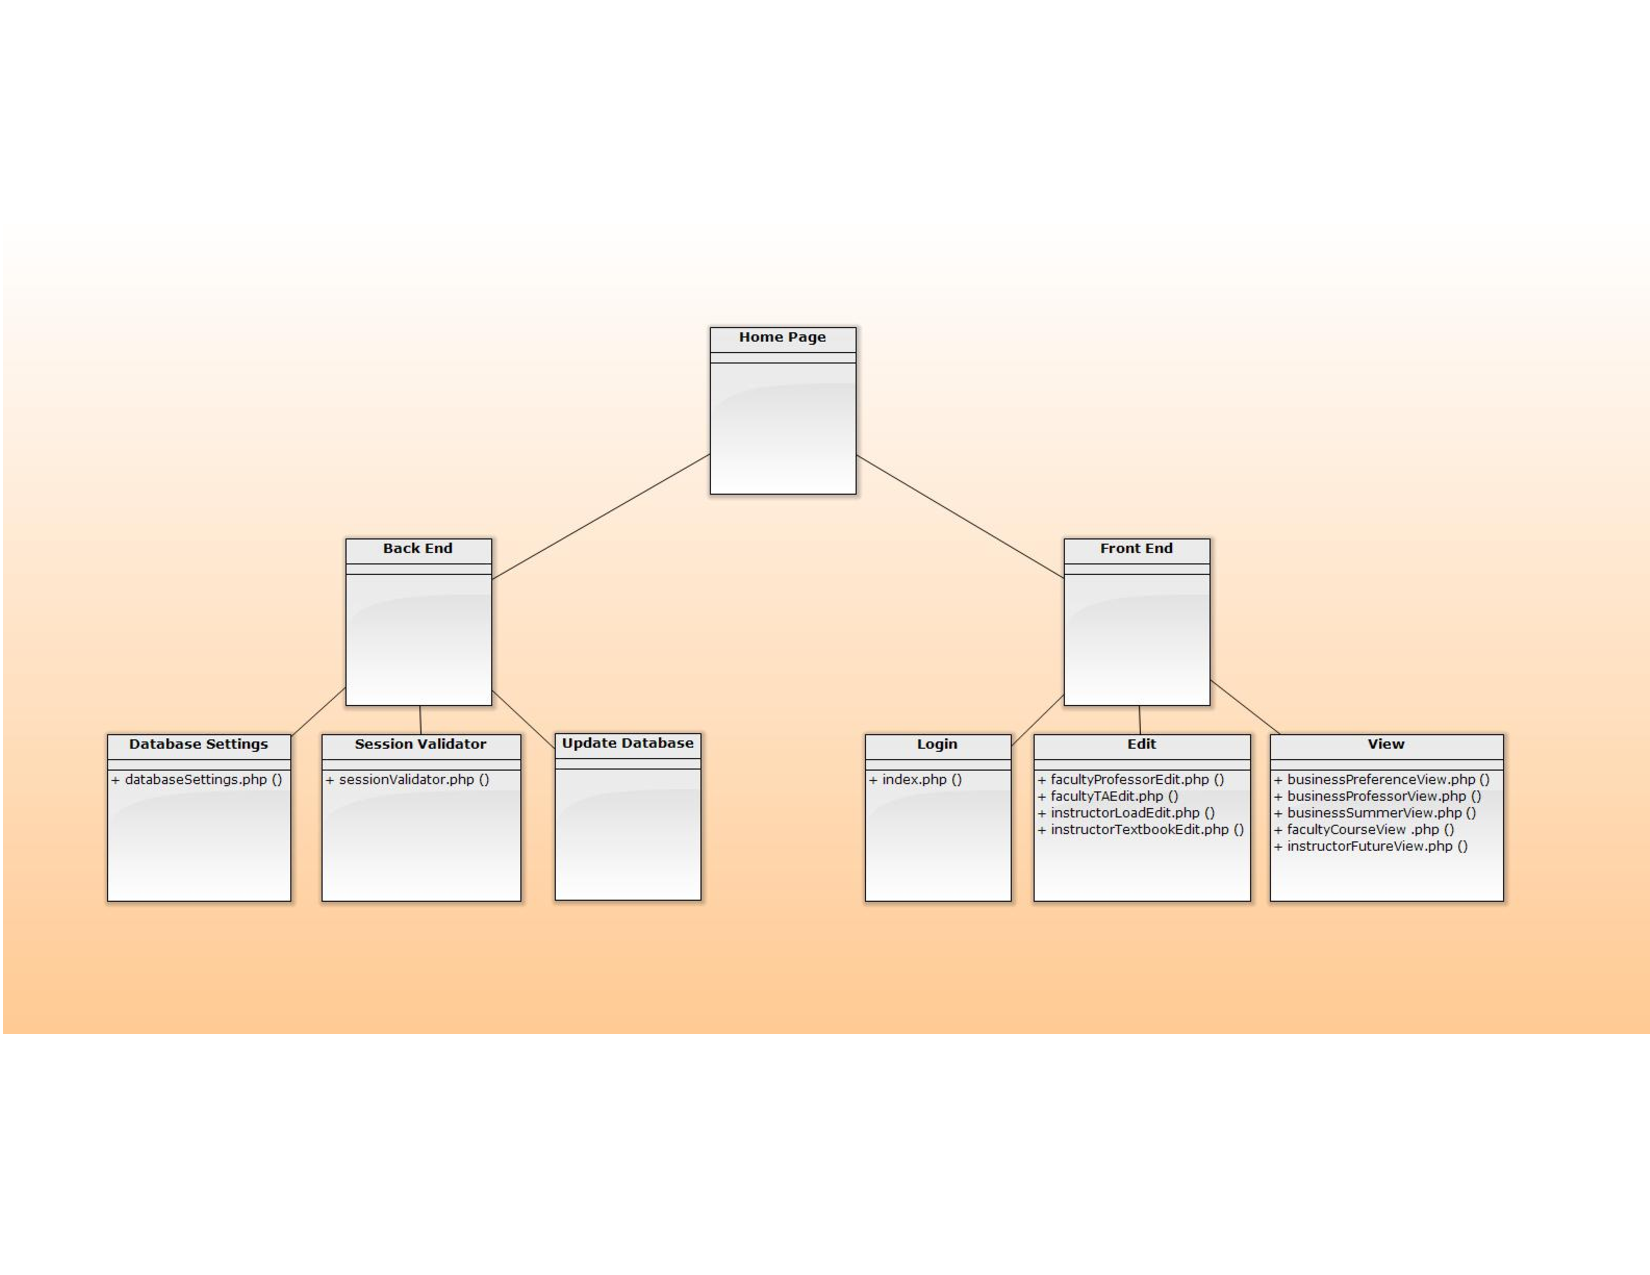
\includepdf[landscape]{design.pdf}  

%Prefers Table	

\section{Home Page}
 The home page consist of a front and back end. The front end is where the application users interact with the page directly. The back end serves indirectly in support of the front end services.
	
	\subsection{Back End}
	The back end serves indirectly in support of the front end, consisting of database settings, session validation and database update applications.
	
		\subsubsection{Database Settings}
		The database settings specifies the host type, username, password, and schema for the database.
		\begin{algorithm}[H]
		\caption{Database Settings}
		\begin{algorithmic}[1]
				\State\textbf{set} host type
				\State\textbf{set} host username 
				\State\textbf{set} host password 
				\State\textbf{set} host schema
		\end{algorithmic}		 
		\end{algorithm}
		
		\subsubsection{Session Validator}
		The session validator checks the rNumber of a user after their login. 
		\begin{algorithm}[H]
		\caption{Session Validator}
		\begin{algorithmic}[1]
		\State start\_session()\Comment{PHP function creates session or resumes session}
		\If{rNumber not valid}
			\State session\_destroy()
			\State exit()
		\Else
			\If{type not valid }
			\State exit()
			\EndIf
		\EndIf
		\end{algorithmic} 
		\end{algorithm}
		
		%\subsubsection{Update Database}	
		%We need something here.
	
	\subsection{Front End}
	The front end is where the application users interact with the page directly, consisting of login, edit and view applications.
		
		\subsubsection{Login}
		The login is the process by which user access to a page is controlled by identifying and authenticating the user's rNumber and password. 
		
		\begin{algorithm}[H]
			\caption{Login}
			\begin{algorithmic}[1]
			\State start\_session()
			\State \textbf{include} database settings
			\State \textbf{include} page layout
			\State \textbf{include} login box
			\If{rNumber and password}
				\State \textbf{get} int value of rNumber
				\If{rNumber $>$ 0}
				\State start connection between SQL and PHP
					\If{no connection error}
					\State \textbf{hash} password
						\If{correct password and rNumber}
					 	\State \textbf{set} expiration time for session
					 		\If{account type == faculty}
					 		\State \textbf{direct} to faculty home page 
					 		\ElsIf{account type == instructor}
					 		\State \textbf{direct} to instructor home page 
					 		\ElsIf{account type == business}
					 		\State \textbf{direct} to business home page
					 		\Else
					 		\State \textbf{diplay} error message: user has invalid account type
					 		\EndIf 	
					 	\Else
					 	\State \textbf{diplay} error message: invalid rNumber or password
					 	\EndIf 
					\Else
				 	\State \textbf{diplay} error message: invalid request
				 	\EndIf 
				\Else
			 	\State \textbf{diplay} error message: unable to connect to database	
				\EndIf
			\Else
			\State \textbf{diplay} error message: invalid rNumber	
			\EndIf			
		\end{algorithmic} 
		\end{algorithm}
		
		\subsubsection{Edit}
		
		The edit page is where the user has access to edit the data of the database according to the user's privileges. In the system a template is used to create all the edit pages, in addition each page is customized according to the system necessities. 
		
		\begin{algorithm}[H]
		\caption{Edit}
			\begin{algorithmic}[1]
			\State \textbf{set} page type to (faculty$|$instructor) 
			\State \textbf{include} database settings
			\State \textbf{include} session validator
			\State \textbf{include} page layout
			\State \textbf{open} connection with database
			\If{No connection error}
				\If{Data to display}
				\State \textbf{create} table
				\EndIf
				\While{Data to fetch}
				\State \textbf{display} data in table
				\EndWhile
			\Else
			\State \textbf{display} error message: failure to connect 
			\EndIf
			\State \textbf{get} user input data
			\State \textbf{update} database
			
			\end{algorithmic}
		\end{algorithm}
		
		\subsubsection{View}
		The view page is where the user has access to view the data of the database. In the system, a template is use to create all the view pages. In addition, each page is customized according to the system necessities. 
		
		\begin{algorithm}[H]
		\caption{View}
			\begin{algorithmic}[1]
			\State \textbf{set} page type to (faculty$|$business$|$instructor) 
			\State \textbf{include} database settings
			\State \textbf{include} session validator
			\State \textbf{include} page layout
			\State \textbf{open} connection with database
			\If{No connection error}
				\If{Data to display}
				\State \textbf{create} table
				\EndIf
				\While{Data to fetch}
				\State \textbf{display} data in table
				\EndWhile
				\State \textbf{close} connection with database
			\Else
			\State error message: failure to connect 
			\EndIf
			\end{algorithmic}
		\end{algorithm}
		
\section{General Webpage}
	\subsection{Glossary}
		\begin{itemize}
			\item AJAX: Asynchronous Javascript And XML – A way for a webpage to be updated dynamically without having to be reloaded.
			\item HTML: HyperText Markup Language – A language for describing the information contained in webpages, as well as the links between them and the visual layout/graphics.
			\item HTTP: HyperText Transfer Protocol – A standard that browsers use to send and receive information to and from web servers.
			\item Javascript – A programming language widely used within web pages, on the client side, to make them more interactive and dynamic.
			\item MySQL – A popular database system, as well as a language for retrieving and storing information in databases.
			\item PHP: PHP Hypertext Preprocessor – A programming language that resides on the server side to create dynamically generated HTML webpages.
			\item Server – A computer that hosts (stores) webpages, communicating with browsers and other entities to allow them to display the webpage's information.
			\item Web Browser – A program that connects to the internet and displays webpages.
			\item XML: eXtensible Markup Language – A language similar to HTML but more general, intended for the storage of any kind of data. Often used in conjunction with programming languages for web interaction (see AJAX)
		\end{itemize}


	\subsection{Typical Interactions with a Webpage}
		\begin{figure}[H]
			\centering
			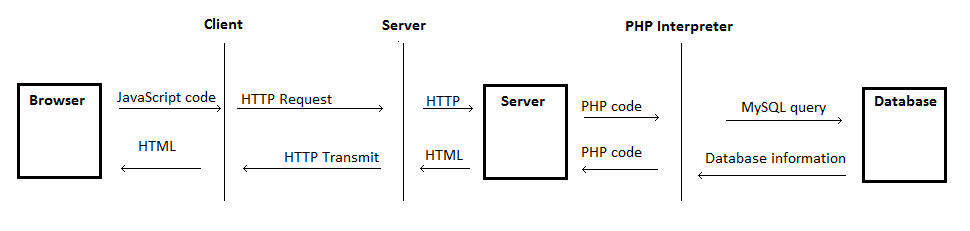
\includegraphics[scale=0.555]{Internet_Diagram.png}
			\caption{Internet Diagram}
		\end{figure}
		\begin{enumerate}
			\item A browser sends an HTTP request to a server, saying it wants the information stored in the webpages.
		
			\item 		The server receives the request. If the request is invalid a code will be transmitted that prompts the browser to display an error message.
		
			\item 		If it is valid, the server performs different operations depending on the contents of the webpage. If the page is an HTML file, it is transmitted as is. If the page is a PHP file or contains PHP code, that code is executed on the server, generating an HTML file that is sent to the user's browser (so the end user never sees the PHP code, only the HTML it generates).
		
			\item 		If the information was correctly received, the browser displays the webpage on the screen for the user to see.
		
			\item 		The user can then interact with the webpage. In our project, this mostly consists of choosing which information should be retrieved from the database and displayed – for instance, a business manager might choose which courses to display information about, or select a certain teacher from a list.

			\item 	Once the user has made a choice, they click a button (or in some other way send a request) and some Javascript code on the page is executed.
	
			\item If the page uses AJAX, the user's choices can be read and changes made to the webpage immediately, without sending a new request and reloading the page.

			\item Otherwise, their choices are transmitted to the server, once again by HTTP request. The server then can run PHP code which uses that information as input to generate HTML code based on the user's requests, which is retransmitted to their browser.

			\item Additionally, PHP code can use MySQL statements or `queries' to retrieve information from within a database on the server, and dynamically place that information into the HTML code the user receives.	

		\end{enumerate}



\chapter{User Interface Design}              
The section covers the basic information regarding template design and specifications. The design templates resembles the Texas Tech website template style. 
\section{Wireframe}
All pages use a standardize background template. The background template contains the Texas Tech University banner on top. The background is divided into three sections, two side sections which are Tech Dark Red and one middle section which is white. The horizontal navigation bar is located at the left side just bellow the banner
\subsection{Sign-In}
The sign-in template contains the standard background template and sign-in box with no navigation bar.
\begin{figure}[h!]
  	\centering
  	
\includegraphics[scale=0.5]{Login.png}
	\caption{Login Page}
\end{figure}

\newpage
\subsection{Edit Template}
The Edit template contains the standard background template and edit table.
\begin{figure}[H]
  	\centering
  	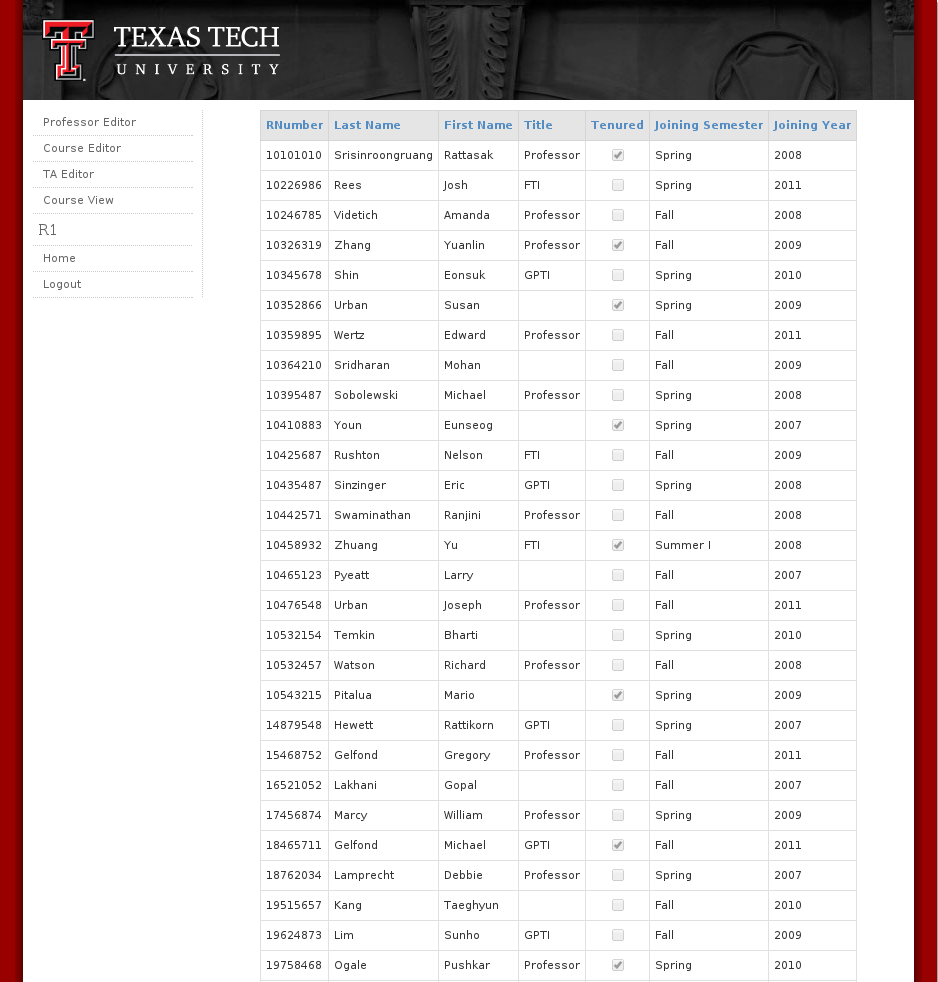
\includegraphics[scale=0.5]{ProfessorEditor.png}
    \caption{Professor Edit Page}
\end{figure}

\newpage
\subsection{View Template}
The view template contains the standard background template and output table.
\begin{figure}[H]
	\centering
	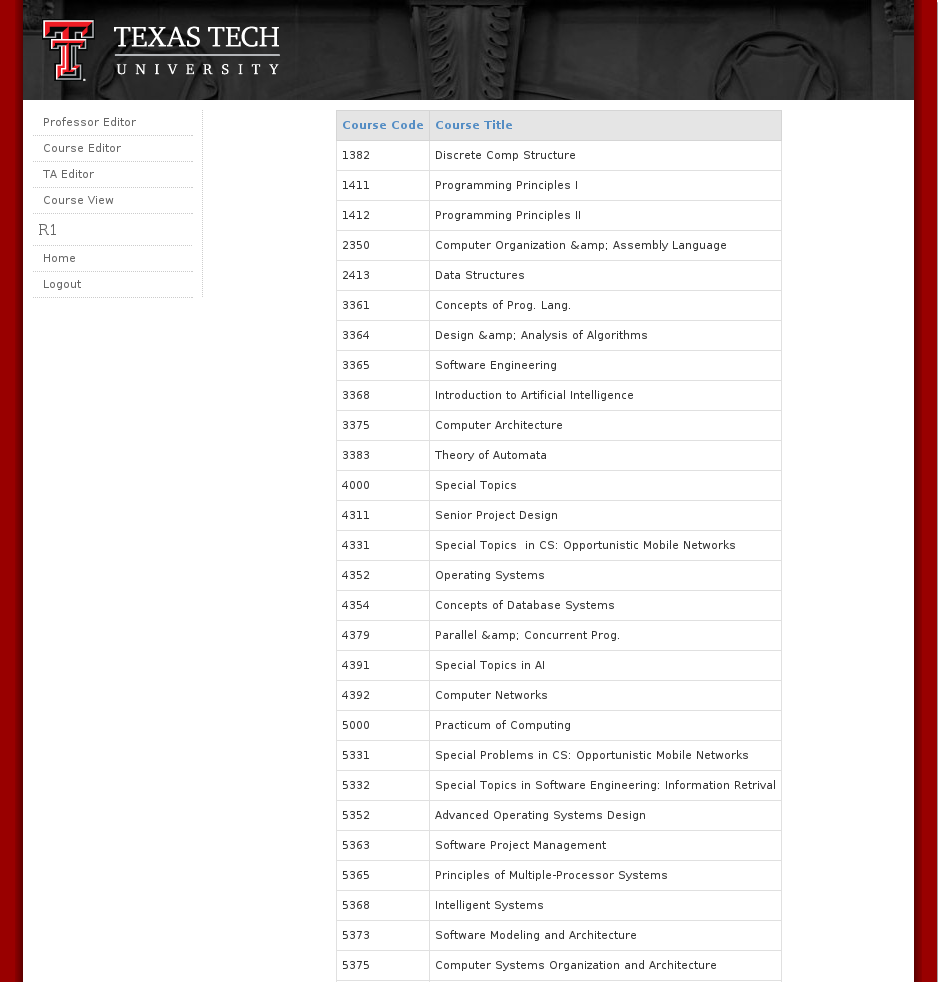
\includegraphics[scale=0.5]{CourseView.png}
	\caption{Course View Page}
\end{figure}
\section{Typography}
The typefaces style has been written to automatically format attractive, readable headers and paragraphs with the following substitutions:\\

\noindent\textbf{High-level headers and some major introductory paragraphs}\\
Arial\\

\noindent\textbf{General content and lower-level headers}\\
Arial

\section{Color}
The page template colors are Texas Tech Dark Red and Texas Tech Black official colors. This is the primary palette used to represent Texas Tech University.	
\begin{figure}[h!]
  	\centering
  	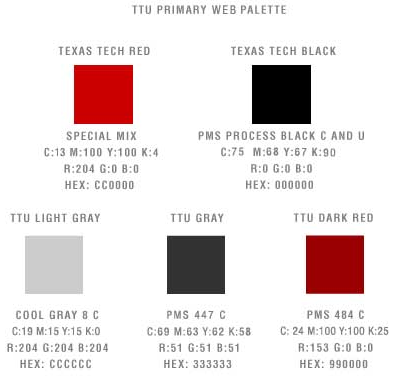
\includegraphics[scale=1]{Capture.PNG}
	\caption{Texas Tech Color Pallet}
\end{figure}

\chapter{Contributions}
\section{Author 1}
\input{author1Contributions.tex}

\section{Author 2}
\input{author2Contributions.tex}

\section{Author 3}
\input{author3Contributions.tex}

\end{document}